\documentclass[12pt]{article}

\usepackage[a4paper,margin=2.5cm]{geometry}
\usepackage{amsmath, amssymb, amsthm}
\usepackage{bm}
\usepackage{hyperref}
\usepackage{graphicx}
\usepackage{caption}
\usepackage{listings}
\usepackage{xcolor}
\usepackage{float}
\usepackage{placeins}
\graphicspath{{figures/}}

\lstdefinestyle{code}{
  basicstyle=\ttfamily\small,
  numbers=left,
  numberstyle=\tiny,
  numbersep=8pt,
  keywordstyle=\color{blue},
  commentstyle=\color{teal!70!black},
  stringstyle=\color{orange!70!black},
  showstringspaces=false,
  breaklines=true,
  frame=single,
  framerule=0.3pt,
  rulecolor=\color{black!15}
}
\lstset{style=code}

\title{Proximal Policy Optimization (PPO) Tutorial}
\author{}
\date{\today}

\begin{document}
\maketitle

\section{Introduction}
Proximal Policy Optimization (PPO) constrains policy updates by clipping the probability ratio between new and old policies, providing a simple and stable on-policy algorithm. PPO balances exploration and stability without the complexity of trust-region constraints.

\section{Theory and Formulas}
\subsection{Clipped Objective}
Given trajectories collected under \(\pi_{\theta_{old}}\), PPO maximizes
\begin{equation}
L^{CLIP}(\theta) = \mathbb{E}\big[ \min( r_t(\theta) \hat{A}_t, \operatorname{clip}(r_t(\theta), 1 - \epsilon, 1 + \epsilon) \hat{A}_t ) \big],
\end{equation}
where \(r_t(\theta) = \frac{\pi_\theta(a_t\mid s_t)}{\pi_{\theta_{old}}(a_t\mid s_t)}\) and \(\hat{A}_t\) is an advantage estimate.

\subsection{Value and Entropy Losses}
The full PPO loss combines policy, value, and entropy terms:
\begin{equation}
L(\theta) = \mathbb{E}\big[ L^{CLIP}(\theta) - c_v (V_\theta(s_t) - \\hat{V}_t)^2 + c_{\text{ent}} H[\pi_\theta(\cdot\mid s_t)] \big].
\end{equation}
Rollouts are typically split into mini-batches, and several epochs of stochastic gradient ascent are performed per batch.

\subsection{Advantage Estimation}
Generalized Advantage Estimation (GAE) reduces variance:
\begin{equation}
\hat{A}_t = \sum_{l=0}^{\infty} (\gamma \lambda)^l \delta_{t+l},\quad \delta_t = r_{t+1} + \gamma V(s_{t+1}) - V(s_t).
\end{equation}
In tabular examples shorter horizons suffice, but GAE remains effective with neural networks.

\section{Applications and Tips}
\begin{itemize}
  \item \textbf{Continuous control}: widely used in robotics and locomotion benchmarks (MuJoCo, Isaac Gym).
  \item \textbf{Large-scale training}: robust under parallel rollout collection and mini-batch updates.
  \item \textbf{Games and simulation}: stable alternative to TRPO with simpler implementation.
  \item \textbf{Best practices}: tune clipping range \(\epsilon\), normalize advantages, anneal learning rate, monitor clip fraction and KL divergence, and use value clipping to prevent critic drift.
\end{itemize}

\section{Python Practice}
The script \texttt{gen\_ppo\_figures.py} trains a tabular PPO agent on a stochastic grid-world. It logs episode returns and the clip fraction (percentage of samples hitting the clipping boundary) to diagnose policy updates.
\begin{lstlisting}[language=Python,caption={Excerpt from gen_ppo_figures.py}]
ratio = np.exp(log_prob_new - log_prob_old)
clipped_ratio = np.clip(ratio, 1 - eps_clip, 1 + eps_clip)
policy_loss = -np.mean(np.minimum(ratio * advantages, clipped_ratio * advantages))
clip_fraction = np.mean((np.abs(ratio - 1.0) > eps_clip/2).astype(float))
\end{lstlisting}

\section{Result}
\begin{figure}[H]
  \centering
  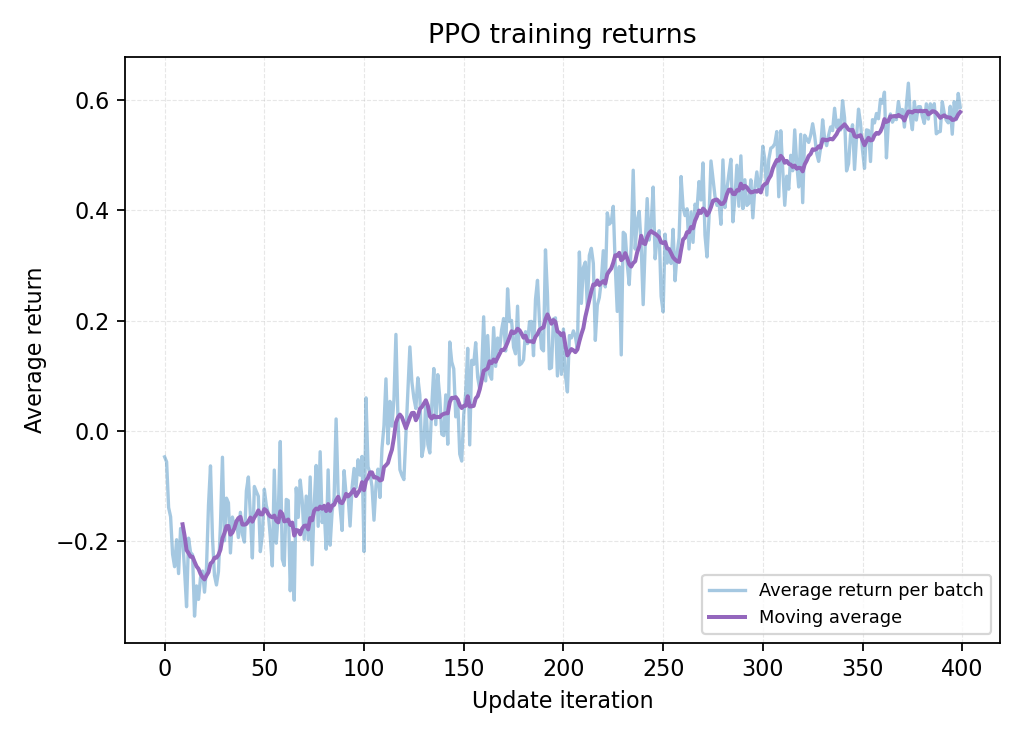
\includegraphics[width=0.8\linewidth]{ppo_returns.png}
  \caption{PPO episode returns over training with moving average smoothing}
  \label{fig:ppo_returns}
\end{figure}

\begin{figure}[H]
  \centering
  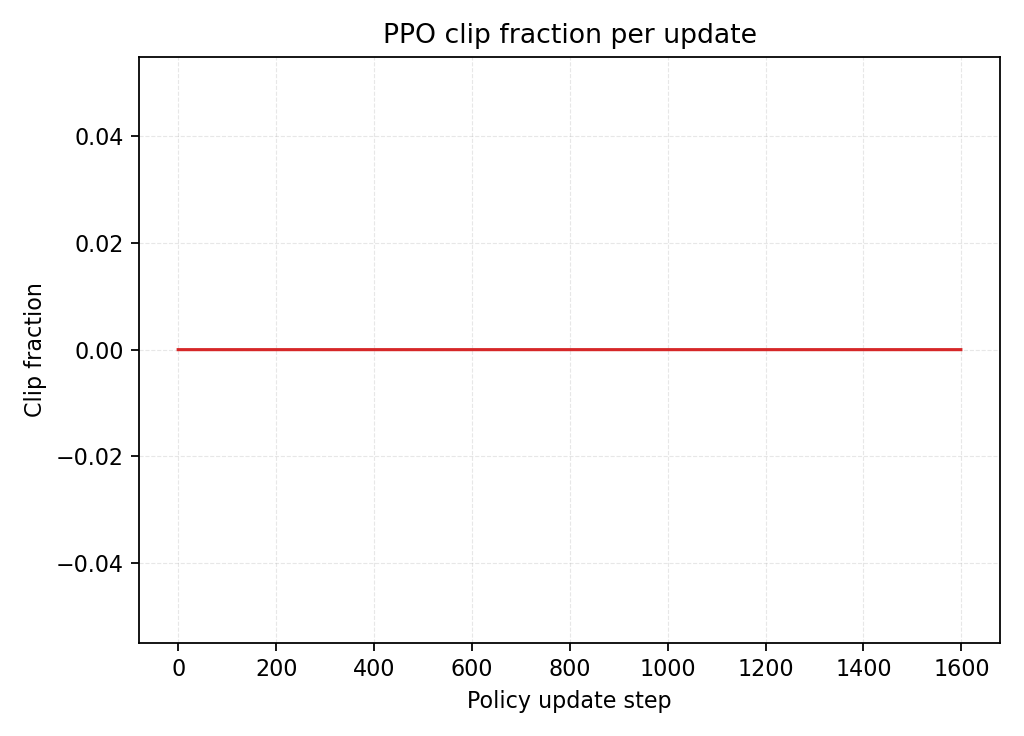
\includegraphics[width=0.82\linewidth]{ppo_clip_stats.png}
  \caption{Clip fraction per update, illustrating how often the policy ratio was truncated}
  \label{fig:ppo_clip_stats}
\end{figure}

\FloatBarrier
\section{Summary}
PPO performs clipped policy updates to achieve stable on-policy learning with minimal tuning. Advantage normalization, entropy bonuses, and monitoring of clip/ KL statistics help maintain reliable convergence. The grid-world example shows returns improving steadily while clip fractions remain well behaved.

\end{document}